\subsection{Componentes Vanilla}

Embora seja uma abstração simplificada, o funcionamento do sistema de redstone apresenta paralelos com circuitos digitais reais, especialmente no que diz respeito à propagação de sinais e controle lógico. 

Esse sistema interno é bem complexo e cheio de detalhes, o que segue é um resumo dos principais conceitos e componentes da redstone, que serão necessários para compreensão do projeto. Para mais detalhes, é recomendável consultar a wiki do jogo \cite{minecraft_wiki_redstone} \cite{minecraft_wiki}.

\subsubsection{Pó de Redstone}

A poeita de redstone atua como meio de transmissão de sinal, análogo a fios em circuitos eletrônicos. Ela transporta um valor de intensidade que varia de 0 a 15, sendo interpretado, em muitos casos, como sinal lógico binário (0 ou 1) ou como hexadecimal (0-15).

A propagação ao longo da poeira é instantânea (0 RT), porém o sinal perde 1 unidade de força a cada bloco percorrido, limitando a transmissão a no máximo 15 blocos sem o uso de repetidores. 

\begin{figure}[H]
   	\centering
   	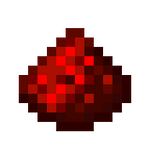
\includegraphics[width=0.2\linewidth]{images/redstone.png}
  	 \caption{Redstone}
   	\label{fig:redstone}
\end{figure}

\subsubsection{Tocha de Redstone}

A tocha de Redstone, além de energizar blocos adjacentes quando está ligada, funciona como um inversor lógico. Quando o bloco em que está apoiada recebe energia, ela desliga; quando não recebe, permanece ligada. Esse comportamento permite a inversão de sinais dentro de circuitos.

\begin{figure}[H]
   	\centering
   	
\includegraphics[width=0.3\linewidth]{images/redstone-torch.png}
  	 \caption{Tocha de Redstone}
   	\label{fig:tocha-de-redstone}
\end{figure}

\subsubsection{Repetidor de Redstone}

O repetidor é um componente multifuncional projetado para transmitir, amplificar e atrasar sinais. Ele possui duas funções avançadas essenciais para o projeto: 

	 \textbf{Ajuste de Delay:} Pode ser configurado manualmente para introduzir um atraso de 1, 2, 3 ou 4 RTs. 

\begin{figure}[H]
   	\centering
   	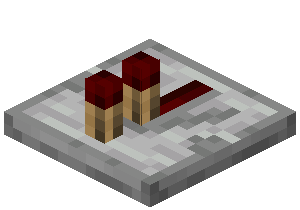
\includegraphics[width=0.3\linewidth]{images/Redstone_Repeater.png}
  	 \caption{Repetidor de Redstone}
   	\label{fig:redstone-repeater}
\end{figure}

	 \textbf{Trava:} Se um repetidor for energizado lateralmente por outro repetidor ou comparador, ele "trava" seu estado atual, ignorando mudanças na entrada traseira. Essa propriedade é frequentemente utilizada para criar memórias de forma compacta.

\begin{figure}[H]
   	\centering
   	
\includegraphics[width=0.34\linewidth]{images/Locked_Redstone_Repeater.png}
  	 \caption{Repetidor de Redstone Travado}
   	\label{fig:locked-redstone-repeater}
\end{figure}

\subsubsection{Comparador de Redstone}

O comparador é o componente mais sofisticado do sistema \textit{vanilla}, permitindo operações aritméticas e de comparação com um atraso constante de 1 RT. Ele opera em dois modos:

 \textbf{Modo Comparação (Tocha frontal apagada):} A saída só é ativada se o sinal traseiro for maior ou igual ao maior sinal lateral. 

\textbf{Modo Subtração (Tocha frontal acesa):} A saída emite uma intensidade igual à diferença entre o sinal traseiro e o maior sinal lateral ($saida = max(0, back - max(side inputs))$). Se o resultado for negativo, a saída é 0.

\begin{figure}[H]
   	\centering
   	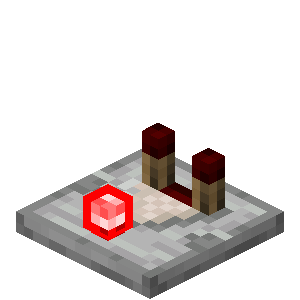
\includegraphics[width=0.34\linewidth]{images/redstone-comparator.png}
  	 \caption{Comparador de Redstone}
   	\label{fig:redstone-comparator}
\end{figure}

\subsubsection{Input/Output}

Componentes como botões, alavancas e placas de pressão atuam como entradas (inputs), fornecendo sinais ao sistema. Já lâmpadas de Redstone e pistões podem ser utilizados como saídas (outputs), respondendo ao estado lógico do circuito.
